
\section{Introduction}
Biological species are well recognised as being engaged in an evolutionary fight-for-survival and Game Theory has been used to analyse the strategies in such a fight.
This kind of analysis is the defining feature of Evolutionary Game Theory, whose many features and concepts are often credited to John Maynard Smith and George R. Price \cite{maynard,maynard2}.
The most standard evolutionary game concerns the continuous growth/decay of organism types; the organism types are defined by the strategy they play as they are continuously randomly paired to participate in a simultaneous symmetric two-player game where the expected payoff determines each participant's growth.\cite{weibull}
However, there is sometimes felt to be a component missing from evolutionary analysis of strategies - the consideration of state.\cite{socialpsyc1,errors1}

Evolutionary game theory has been a valuable tool in characterising the dynamics and interactions among biological species and it also has proven utility in other fields which feature evolutionary dynamics.  Some examples of phenomena which have been modeled via Evolutionary Game Theory include: altruism, empathy, human culture, moral behavior, private property, proto-linguistic behavior, social learning, societal norms, personality and mating-dynamics \cite{sep-game-evolutionary,socialpsyc1,Hodgson2012,McNamara953}.

However, many organisms exhibit behaviors and strategies which are intrinsically coupled with state and hence cannot be directly modeled using standard evolutionary game theory.
Simple and canonical examples include the behavior of perspiring with increasing body temperature causing dehydration, foraging behavior with hunger signals causing food shortage, sleep with ambient light levels causing vulnerability to predation, or hibernation with the change of season causing hunger.

Within this paper we detail an evolutionary game for modeling stateful evolutionary dynamics and an algorithm which solves for its equilibria. We give a simple demonstration of the game via an extension of the classic Hawk-Dove game\cite{maynard} and we compare the game with the approach of others.

\subsection{Related Work}
Complex state-action interactions between individuals can always be stochastically modeled by artificial life simulations.\cite{alife1} But recent work has been conducted to incorporate some state-action dynamics into the exacting mathematical framework of evolutionary game theory.

This work has developed along two different branches, the first branch consists of encoding the organisms as belonging to nodes on a graph structure.\cite{spacial4} In this approach the organisms at a node play the symmetric game against weighted probabilities of their nearest neighbors and/or themself. Such games are called `Spacial Evolutionary Games'\cite{spacial1,nowak} and they have unique and dynamic behavior\cite{spacial2,spacial3}. Spacial Evolutionary Games feature the addition of specifying a `who-plays-with-who' into the game structure but the game itself is the same for all the participants.
Spacial Evolutionary Games are apt to model the evolution of organism's strategies between strategic nodes but it is seen to fail to capture the organisms having state beyond generalised location.

The second approach is more recent and consists of integrating state (and transitions between state) into the symmetric two-player game itself. This pioneering effort has centered around the works of Eitan Altman, and his colleagues Ilaria Brunetti and Yezekael Hayel \cite{markov2,markov3,markov4,markov5,markov8,markov9}, who introduce the Markov-Decision-Evolutionary-Game (MDEG) and variants thereof.

An MDEG consists in analysing the growth/decay of organism-types in a population where the organisms can occupy a finite set of states. The organism-types are defined by the strategy they play of choosing actions depending on their state as they are continuously randomly paired to participate in a two-player symmetric game. The game consists of each participant choosing an action and the game's outcomes depend on the chosen actions and the states of the participants. The game's outcomes determine the instantaneous payoff and probable transition to other states experienced by the participants. The expected long-term payoff determines the growth/decay of the organism-types which then changes the composition of the population in which the game is played.

Several example MDEG games are introduced in Altman's literature including modifications and extensions of the Hawk-Dove game from which we take inspiration.\cite{markov3,markov5}
MDEG includes many features for modeling state-action interactions within evolutionary game theory and serves to provide a contrast for our game. By our game, we show that by relaxing the markov nature of MDEG we allow a remarkably more flexible game, a game which features other evolutionary games as subtypes.

\subsection{Structure}
The remainder of this paper is organised as follows: section \ref{sec:2} presents the core concept of non-markovian transmission of organisms between states, section \ref{section:formalism} gives formalism to the non-markovian game and its algorithm, section \ref{sec:equilibria} discusses the game's equilibria and gives confinement for the algorithm's equilibria search, section \ref{sec:example} details a Hawk-Dove game as example of the working algorithm, and section \ref{sec:discussion} concludes the paper by evaluating and comparing the features of our game.

\section{Non-Markov population models}\label{sec:2}

The demographic flow of individuals of a species' population between states is sometimes described in ecological-studies by a matrix that is not necessarily markov.\cite{population1}
The simplest example of such matrices are Leslie Matrices used for studying the structure of populations of individuals transitioning between evenly spaced age-states.
Leslie Matrices are square, and they have form \cite{leslie}:

\begin{equation*}
M=\begin{bmatrix}
    F_0 & F_1 & F_2 & \dots  & F_{m-2} & F_{m-1} & F_m  \\
    P_0 &  0  &  0  & \dots  &    0    &  0      &  0   \\
     0  & P_1 &  0  & \dots  &    0    &  0      &  0   \\
     0  &  0  & P_2 & \dots  &    0    &  0      &  0   \\
    \vdots & \vdots & \vdots & \ddots & \vdots & \vdots & \vdots \\
     0  &  0  &  0  & \dots  & P_{m-2} &  0      &  0   \\
     0  &  0  &  0  & \dots  &    0    & P_{m-1} &  0   \\
\end{bmatrix}
~~~0<P_x<1;~~F_x\ge0
\end{equation*}
Where $P_i$ represents the probability of and individual in the $i$th age bracket successfully living into the $(i+1)$th age bracket, and $F_i$ is average number of offspring for an individual in $i$th age bracket within the duration of the age bracket.
For a column vector $n = [n_0,n_1,n_2,\dots,n_m]$ with each $n_i$ representing the number of individuals in each age-bracket, $Mn$ gives the expected number of individuals in the population after the duration of one age bracket of time, and $M^2n$ the expectation individuals after two age brackets, $M^3n$ after three, and so on.
Successive applications eventually yield a steady population profile between the $n_i$, and a constant exponential growth rate $\lambda$ given by the Euler–Lotka equation.
The $\lambda$ is the dominant and only real-positive eigenvalue of the matrix, with the steady distribution $n$ as its corresponding eigenvector, that is $Mn=\lambda n$.

Although the elements in the Leslie matrix are positive and represent states of organisms in the population and the transition between, the matrix isn't Markov because its columns don't necessarily sum to one.  The informal difference is that whereas in a Markov-chain matrix the elements represent the expectation of \textit{transition} between states, Leslie matrix elements represent the expectation of \textit{transmission} between states inclusive of such possible factors as births and deaths.
We term the class of such matrices as `transmission matrices' in this article and assert the only thing defining such matrices are that they are real, square and have non-negative elements.\footnote{General non-negative real square matrices (or at-least irreducible ones) have at-least one real non-negative eigenvalue (via indirect application of Perron-Frobenius theorem, see chapter 3 of \cite{matrix2}) hence a transmission matrix identifies at-least one growth-rate}
We do this because such matrices can be built more broadly than simple Leslie-matrix form\cite{models1,models2}. Consider the rich interaction between organism-states captured by the matrix of transmissions for the 'Nodding Thistle' in figure \ref{fig:1}.



\begin{figure}[h]
    \begin{subfigure}[b]{.5\linewidth}
        \centering
        \begin{tikzpicture}[scale=0.9, transform shape,->,>=stealth',shorten >=1pt,auto,node distance=1.7cm,thick,main node/.style={circle}]
            \path[use as bounding box] (-2.5cm, -2.8cm) rectangle (2.5cm, 2.5cm);
            \node[main node] (SB)  at (-2cm,  2cm) [align=center, text width=2.1cm] {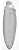
\includegraphics[width=.05\textwidth]{1.png}\\\small Seed};
            \node[main node] (SM)  at ( 2cm,  2cm) [align=center, text width=2.1cm] {
\includegraphics[width=.25\textwidth]{2.png}\\\small Small};
            \node[main node] (ME)  at ( 2cm, -2cm) [align=center, text width=2.1cm] {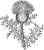
\includegraphics[width=.29\textwidth]{3.png}\\\small Medium};
            \node[main node] (LE)  at (-2cm, -2cm) [align=center, text width=2.1cm] {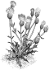
\includegraphics[width=.38\textwidth]{4.png}\\\small Large};

            \node[main node] (SBm) at (-2cm,  2cm) [align=center, text width=1.2cm] {};
            \node[main node] (SMm) at ( 2cm,  2cm) [align=center, text width=1.2cm] {};
            \node[main node] (MEm) at ( 2cm, -2cm) [align=center, text width=1.2cm] {};
            \node[main node] (LEm) at (-2cm, -2cm) [align=center, text width=1.2cm] {};

            \path[every node/.style={sloped,auto=false}]
            (SBm) edge [in=180-20,out=180+20,looseness=3,   line width=1pt,anchor=south] node  {\scriptsize 0.443} (SBm)
            (SBm) edge [bend left=15,                       line width=1pt,anchor=south] node  {\scriptsize 0.0039} (SMm)
            (SBm) edge [bend left=15,                       line width=1pt,anchor=south] node  {\scriptsize 0.0004} (MEm)
            (SBm) edge [bend left=15,                       line width=1pt,anchor=south] node  {\scriptsize 0.0005} (LEm)

            (SMm) edge [bend left=15,                       line width=1pt,anchor=south] node  {\scriptsize 0.1584} (SBm)
            (SMm) edge [in=20,out=-20,looseness=3,          line width=1pt,anchor=north] node  {\scriptsize 0.0078} (SMm)
            (SMm) edge [bend left=15,                       line width=1pt,anchor=south] node  {\scriptsize 0.0031} (MEm)
            (SMm) edge [bend left=15,                       line width=1pt,anchor=north] node  {\scriptsize 0.01} (LEm)

            (MEm) edge [bend left=15,                       line width=1pt,anchor=north] node  {\scriptsize 6.6105} (SBm)
            (MEm) edge [bend left=15,                       line width=1pt,anchor=south] node  {\scriptsize 0.2434} (SMm)
            (MEm) edge [in=-20,out=20,looseness=3,          line width=1pt,anchor=south] node  {\scriptsize 0.0314} (MEm)
            (MEm) edge [bend left=15,                       line width=1pt,anchor=south] node  {\scriptsize 0.0613} (LEm)

            (LEm) edge [bend left=15,                       line width=1pt,anchor=south] node  {\scriptsize 206.56} (SBm)
            (LEm) edge [bend left=15,                       line width=1pt,anchor=south] node  {\scriptsize 7.6091} (SMm)
            (LEm) edge [bend left=15,                       line width=1pt,anchor=south] node  {\scriptsize 0.793} (MEm)
            (LEm) edge [in=180+20,out=180-20,looseness=3,   line width=1pt,anchor=north] node  {\scriptsize 0.945} (LEm)
            ;
        \end{tikzpicture}

        \caption{Life cycle graph of the population model}\label{fig:1a}
    \end{subfigure}
    \begin{subfigure}[b]{.5\linewidth}
        \centering
        \footnotesize
        $$ \begin{bmatrix}\text{Seed}_{t+1}\\\text{Small}_{t+1}\\\text{Medium}_{t+1}\\\text{Large}_{t+1}\end{bmatrix}= 
        \begin{bmatrix}
            0.443&0.1584&6.6105&206.56\\
            0.039&0.0078&0.2434&7.6091\\
            0.0004&0.0031&0.0314&0.793\\
            0.0005&0.01&0.0613&0.945
        \end{bmatrix}
        \begin{bmatrix}\text{Seed}_{t}\\\text{Small}_{t}\\\text{Medium}_{t}\\\text{Large}_{t}\end{bmatrix}$$
        \caption{
            4x4 matrix model of a Nodding Thistle (\textit{Carduus nutans}) population in Australia, classification based on seed and rosette size. The transmission numbers represent aggregate survival/growth/propagation of individuals from one class into another per year. The projected population growth rate ($\lambda$) is 1.207 per year.\\
      Data from Jongejans et.al\cite{models2}\\ Original data from Shea et.al\cite{models3}
        }\label{fig:1b}
    \end{subfigure}
        \vspace{-2.3\baselineskip}
    \caption{}\label{fig:1}
\end{figure}

It is by these transmission matrices that we are able to highlight the notion of transmission between two states as being the demographic flow of the population from one to the other.
This notion forms a core concept in the next section as we introduce actions for the organisms and thence compare strategies in game-theory analysis for equilibria.

